%==========================================
%
% SIBGRAPI 2026 paper template
% Example of IEEEtran.cls
%
%==========================================

% *** Authors should verify (and, if needed, correct) their LaTeX system  ***
% *** with the testflow diagnostic prior to trusting their LaTeX platform ***
% *** with production work. The IEEE's font choices and paper sizes can   ***
% *** trigger bugs that do not appear when using other class files.       ***                          ***
% The testflow support page is at:
% http://www.michaelshell.org/tex/testflow/

\documentclass[10pt,conference]{IEEEtran}


% Some very useful LaTeX packages include:
% (uncomment the ones you want to load)


% *** MISC UTILITY PACKAGES ***
%
%\usepackage{ifpdf}
% Heiko Oberdiek's ifpdf.sty is very useful if you need conditional
% compilation based on whether the output is pdf or dvi.
% usage:
% \ifpdf
%   % pdf code
% \else
%   % dvi code
% \fi
% The latest version of ifpdf.sty can be obtained from:
% http://www.ctan.org/pkg/ifpdf
% Also, note that IEEEtran.cls V1.7 and later provides a builtin
% \ifCLASSINFOpdf conditional that works the same way.
% When switching from latex to pdflatex and vice-versa, the compiler may
% have to be run twice to clear warning/error messages.






% *** CITATION PACKAGES ***
%
\usepackage{cite}
% cite.sty was written by Donald Arseneau
% V1.6 and later of IEEEtran pre-defines the format of the cite.sty package
% \cite{} output to follow that of the IEEE. Loading the cite package will
% result in citation numbers being automatically sorted and properly
% "compressed/ranged". e.g., [1], [9], [2], [7], [5], [6] without using
% cite.sty will become [1], [2], [5]--[7], [9] using cite.sty. cite.sty's
% \cite will automatically add leading space, if needed. Use cite.sty's
% noadjust option (cite.sty V3.8 and later) if you want to turn this off
% such as if a citation ever needs to be enclosed in parenthesis.
% cite.sty is already installed on most LaTeX systems. Be sure and use
% version 5.0 (2009-03-20) and later if using hyperref.sty.
% The latest version can be obtained at:
% http://www.ctan.org/pkg/cite
% The documentation is contained in the cite.sty file itself.






% *** GRAPHICS RELATED PACKAGES ***
%
\ifCLASSINFOpdf
   \usepackage[pdftex]{graphicx}
  % declare the path(s) where your graphic files are
   \graphicspath{{figs/}}
  % and their extensions so you won't have to specify these with
  % every instance of \includegraphics
   \DeclareGraphicsExtensions{.pdf,.jpeg,.png}
\else
  % or other class option (dvipsone, dvipdf, if not using dvips). graphicx
  % will default to the driver specified in the system graphics.cfg if no
  % driver is specified.
   \usepackage[dvips]{graphicx}
  % declare the path(s) where your graphic files are
   \graphicspath{{../figs/}}
  % and their extensions so you won't have to specify these with
  % every instance of \includegraphics
   \DeclareGraphicsExtensions{.eps}
\fi
% graphicx was written by David Carlisle and Sebastian Rahtz. It is
% required if you want graphics, photos, etc. graphicx.sty is already
% installed on most LaTeX systems. The latest version and documentation
% can be obtained at: 
% http://www.ctan.org/pkg/graphicx
% Another good source of documentation is "Using Imported Graphics in
% LaTeX2e" by Keith Reckdahl which can be found at:
% http://www.ctan.org/pkg/epslatex
%
% latex, and pdflatex in dvi mode, support graphics in encapsulated
% postscript (.eps) format. pdflatex in pdf mode supports graphics
% in .pdf, .jpeg, .png and .mps (metapost) formats. Users should ensure
% that all non-photo figures use a vector format (.eps, .pdf, .mps) and
% not a bitmapped formats (.jpeg, .png). The IEEE frowns on bitmapped formats
% which can result in "jaggedy"/blurry rendering of lines and letters as
% well as large increases in file sizes.
%
% You can find documentation about the pdfTeX application at:
% http://www.tug.org/applications/pdftex





% *** MATH PACKAGES ***
%
\usepackage[cmex10]{amsmath}
% A popular package from the American Mathematical Society that provides
% many useful and powerful commands for dealing with mathematics.
%
% Note that the amsmath package sets \interdisplaylinepenalty to 10000
% thus preventing page breaks from occurring within multiline equations. Use:
\interdisplaylinepenalty=2500
% after loading amsmath to restore such page breaks as IEEEtran.cls normally
% does. amsmath.sty is already installed on most LaTeX systems. The latest
% version and documentation can be obtained at:
% http://www.ctan.org/pkg/amsmath
\usepackage{amsthm}
\newtheorem{definition}{Definition}




% *** SPECIALIZED LIST PACKAGES ***
%
\usepackage{algorithmic}
% algorithmic.sty was written by Peter Williams and Rogerio Brito.
% This package provides an algorithmic environment fo describing algorithms.
% You can use the algorithmic environment in-text or within a figure
% environment to provide for a floating algorithm. Do NOT use the algorithm
% floating environment provided by algorithm.sty (by the same authors) or
% algorithm2e.sty (by Christophe Fiorio) as the IEEE does not use dedicated
% algorithm float types and packages that provide these will not provide
% correct IEEE style captions. The latest version and documentation of
% algorithmic.sty can be obtained at:
% http://www.ctan.org/pkg/algorithms
% Also of interest may be the (relatively newer and more customizable)
% algorithmicx.sty package by Szasz Janos:
% http://www.ctan.org/pkg/algorithmicx




% *** ALIGNMENT PACKAGES ***
%
\usepackage{array}
% Frank Mittelbach's and David Carlisle's array.sty patches and improves
% the standard LaTeX2e array and tabular environments to provide better
% appearance and additional user controls. As the default LaTeX2e table
% generation code is lacking to the point of almost being broken with
% respect to the quality of the end results, all users are strongly
% advised to use an enhanced (at the very least that provided by array.sty)
% set of table tools. array.sty is already installed on most systems. The
% latest version and documentation can be obtained at:
% http://www.ctan.org/pkg/array


% IEEEtran contains the IEEEeqnarray family of commands that can be used to
% generate multiline equations as well as matrices, tables, etc., of high
% quality.




% *** SUBFIGURE PACKAGES ***
\ifCLASSOPTIONcompsoc
  \usepackage[caption=false,font=normalsize,labelfont=sf,textfont=sf]{subfig}
\else
  \usepackage[caption=false,font=footnotesize]{subfig}
\fi
% subfig.sty, written by Steven Douglas Cochran, is the modern replacement
% for subfigure.sty, the latter of which is no longer maintained and is
% incompatible with some LaTeX packages including fixltx2e. However,
% subfig.sty requires and automatically loads Axel Sommerfeldt's caption.sty
% which will override IEEEtran.cls' handling of captions and this will result
% in non-IEEE style figure/table captions. To prevent this problem, be sure
% and invoke subfig.sty's "caption=false" package option (available since
% subfig.sty version 1.3, 2005/06/28) as this is will preserve IEEEtran.cls
% handling of captions.
% Note that the Computer Society format requires a larger sans serif font
% than the serif footnote size font used in traditional IEEE formatting
% and thus the need to invoke different subfig.sty package options depending
% on whether compsoc mode has been enabled.
%
% The latest version and documentation of subfig.sty can be obtained at:
% http://www.ctan.org/pkg/subfig




% *** FLOAT PACKAGES ***
%
%\usepackage{fixltx2e}
% fixltx2e, the successor to the earlier fix2col.sty, was written by
% Frank Mittelbach and David Carlisle. This package corrects a few problems
% in the LaTeX2e kernel, the most notable of which is that in current
% LaTeX2e releases, the ordering of single and double column floats is not
% guaranteed to be preserved. Thus, an unpatched LaTeX2e can allow a
% single column figure to be placed prior to an earlier double column
% figure.
% Be aware that LaTeX2e kernels dated 2015 and later have fixltx2e.sty's
% corrections already built into the system in which case a warning will
% be issued if an attempt is made to load fixltx2e.sty as it is no longer
% needed.
% The latest version and documentation can be found at:
% http://www.ctan.org/pkg/fixltx2e


%\usepackage{stfloats}
% stfloats.sty was written by Sigitas Tolusis. This package gives LaTeX2e
% the ability to do double column floats at the bottom of the page as well
% as the top. (e.g., "\begin{figure*}[!b]" is not normally possible in
% LaTeX2e). It also provides a command:
%\fnbelowfloat
% to enable the placement of footnotes below bottom floats (the standard
% LaTeX2e kernel puts them above bottom floats). This is an invasive package
% which rewrites many portions of the LaTeX2e float routines. It may not work
% with other packages that modify the LaTeX2e float routines. The latest
% version and documentation can be obtained at:
% http://www.ctan.org/pkg/stfloats
% Do not use the stfloats baselinefloat ability as the IEEE does not allow
% \baselineskip to stretch. Authors submitting work to the IEEE should note
% that the IEEE rarely uses double column equations and that authors should try
% to avoid such use. Do not be tempted to use the cuted.sty or midfloat.sty
% packages (also by Sigitas Tolusis) as the IEEE does not format its papers in
% such ways.
% Do not attempt to use stfloats with fixltx2e as they are incompatible.
% Instead, use Morten Hogholm'a dblfloatfix which combines the features
% of both fixltx2e and stfloats:
%
% \usepackage{dblfloatfix}
% The latest version can be found at:
% http://www.ctan.org/pkg/dblfloatfix




% *** PDF, URL AND HYPERLINK PACKAGES ***
%
\usepackage{url}
% url.sty was written by Donald Arseneau. It provides better support for
% handling and breaking URLs. url.sty is already installed on most LaTeX
% systems. The latest version and documentation can be obtained at:
% http://www.ctan.org/pkg/url
% Basically, \url{my_url_here}.




% *** Do not adjust lengths that control margins, column widths, etc. ***
% *** Do not use packages that alter fonts (such as pslatex).         ***
% There should be no need to do such things with IEEEtran.cls V1.6 and later.
% (Unless specifically asked to do so by the journal or conference you plan
% to submit to, of course. )


% correct bad hyphenation here
\hyphenation{op-tical net-works semi-conduc-tor}

%------------------------------------------------------------------------- 
% change the % on next lines to produce the final camera-ready version 
\newif\iffinal
\finalfalse
%\finaltrue
\newcommand{\cmtid}{99999}
%------------------------------------------------------------------------- 

\iffinal
\else
\usepackage[switch]{lineno}
\fi

\begin{document}
%
% paper title
% Titles are generally capitalized except for words such as a, an, and, as,
% at, but, by, for, in, nor, of, on, or, the, to and up, which are usually
% not capitalized unless they are the first or last word of the title.
% Linebreaks \\ can be used within to get better formatting as desired.
% Do not put math or special symbols in the title.
\title{Automatic Prostate Cancer Classification in Whole Slide Images using EfficientNet and Entropy-based Data Filtering}


% author names and affiliations
% use a multiple column layout for up to two different
% affiliations

\iffinal

% author names and affiliations
% use a multiple column layout for up to three different
% affiliations
\author{\IEEEauthorblockN{Michael Shell}
\IEEEauthorblockA{School of Electrical and\\Computer Engineering\\
Georgia Institute of Technology\\
Atlanta, Georgia 30332--0250\\
Email: http://www.michaelshell.org/contact.html}
\and
\IEEEauthorblockN{Homer Simpson}
\IEEEauthorblockA{Twentieth Century Fox\\
Springfield, USA\\
Email: homer@thesimpsons.com}
\and
\IEEEauthorblockN{James Kirk\\ and Montgomery Scott}
\IEEEauthorblockA{Starfleet Academy\\
San Francisco, California 96678--2391\\
Telephone: (800) 555--1212\\
Fax: (888) 555--1212}}

% conference papers do not typically use \thanks and this command
% is locked out in conference mode. If really needed, such as for
% the acknowledgment of grants, issue a \IEEEoverridecommandlockouts
% after \documentclass

% for over three affiliations, or if they all won't fit within the width
% of the page, use this alternative format:
% 
%\author{\IEEEauthorblockN{Michael Shell\IEEEauthorrefmark{1},
%Homer Simpson\IEEEauthorrefmark{2},
%James Kirk\IEEEauthorrefmark{3}, 
%Montgomery Scott\IEEEauthorrefmark{3} and
%Eldon Tyrell\IEEEauthorrefmark{4}}
%\IEEEauthorblockA{\IEEEauthorrefmark{1}School of Electrical and Computer Engineering\\
%Georgia Institute of Technology,
%Atlanta, Georgia 30332--0250\\ Email: see http://www.michaelshell.org/contact.html}
%\IEEEauthorblockA{\IEEEauthorrefmark{2}Twentieth Century Fox, Springfield, USA\\
%Email: homer@thesimpsons.com}
%\IEEEauthorblockA{\IEEEauthorrefmark{3}Starfleet Academy, San Francisco, California 96678-2391\\
%Telephone: (800) 555--1212, Fax: (888) 555--1212}
%\IEEEauthorblockA{\IEEEauthorrefmark{4}Tyrell Inc., 123 Replicant Street, Los Angeles, California 90210--4321}}

\else
  \author{SIBGRAPI Paper ID: \cmtid \\ }
  \linenumbers
\fi


% make the title area
\maketitle

% As a general rule, do not put math, special symbols or citations
% in the abstract
\begin{abstract}
The accurate grading of prostate cancer in whole-slide images (WSIs) is essential for patient prognosis and treatment planning. However, the International Society of Urological Pathology (ISUP) grading system suffers from significant inter-observer variability. In this work, we propose an automated classification system based on the EfficientNet architecture. We investigate the impact of different model scales and propose a novel data filtering strategy based on Shannon entropy to remove non-informative and noisy patches from the training set. Our results demonstrate that the EfficientNet-B0 model, combined with entropy filtering, achieves a Quadratic Weighted Kappa (QWK) of 0.8730, outperforming larger architectures and the baseline model. We also evaluate the impact of alternative color spaces and self-attention mechanisms, finding that standard RGB and local attention (SE blocks) remain the most effective for this task.
\end{abstract}

% no keywords




% For peerreview papers, this IEEEtran command inserts a page break and
% creates the second title. It will be ignored for other modes.
\IEEEpeerreviewmaketitle



\section{Introduction}
Prostate cancer is one of the most common malignancies in men worldwide. The histological grading of prostate biopsies using the ISUP system is the gold standard for assessing disease aggressiveness. Despite its clinical importance, manual grading is subjective, time-consuming, and requires highly specialized pathologists \cite{bulten2020automated}.

Recent advances in deep learning (DL) have shown great promise in automating the analysis of digital pathology slides. Convolutional Neural Networks (CNNs), such as EfficientNet \cite{tan2019efficientnet} and ResNet \cite{he2016deep}, have achieved state-of-the-art performance in various medical imaging tasks. However, digital pathology poses unique challenges, including the massive size of Whole Slide Images (WSIs), the presence of artifacts, and the limited amount of labeled data.

In this paper, we present a comprehensive study on the automated classification of prostate cancer grades using the PANDA Challenge dataset \cite{panda2020}. Our main contributions are:
\begin{itemize}
    \item A systematic evaluation of EfficientNet variants (B0 to B7) for ISUP grading.
    \item A novel entropy-based data filtering method that improves model performance by removing noisy training samples.
    \item An analysis of the effectiveness of alternative color spaces and self-attention mechanisms in histopathology.
\end{itemize}

The remainder of this paper is organized as follows: Section II discusses related work. Section III describes the methodology and experimental setup. Section IV presents the experimental results. Section V provides a comparative analysis of the various strategies. Section VI discusses the findings, and Section VII concludes the work.

\section{Related Work}
The automation of histological grading has been a subject of intense research. Traditional methods relied on handcrafted features such as nuclear morphology and gland texture. However, the complexity and variability of H\&E stained slides made these approaches difficult to generalize.

Deep learning has revolutionized this field. Bulten et al. \cite{bulten2020automated} developed a DL system that achieved performance comparable to expert pathologists in Gleason grading. Their work emphasized the use of large-scale datasets and robust architectures. Similarly, Nagpal et al. demonstrated that DL models can reduce inter-observer variability and improve the consistency of ISUP grading in clinical settings.

EfficientNet architectures \cite{tan2019efficientnet} have recently emerged as a popular choice for medical imaging due to their principled scaling of depth, width, and resolution. While larger models often perform better on natural image datasets like ImageNet, recent studies in digital pathology suggest that smaller, more efficient models can be more robust against the high-frequency noise and artifacts typical of whole-slide imaging. Our work builds upon these findings by specifically investigating the impact of model scale and proposing a novel entropy-based noise reduction strategy.

\section{Methodology}
\subsection{Dataset and Preprocessing}
We utilized the PANDA Challenge dataset \cite{panda2020}, consisting of 10,616 whole-slide images of prostate biopsies. The slides were tiled into smaller patches of $224 \times 224$ pixels. For training, we used a subset of 7,219 images, with 1,805 images for validation (fold 3) and 1,592 for testing.

To improve the model's robustness, we applied extensive data augmentation during training. This included geometric transformations such as random horizontal and vertical flips ($p=0.5$), transpositions ($p=0.5$), and rotations ($p=0.5$). We also incorporated color jittering to account for staining variations between different medical centers.

\subsection{Model Architecture}
The primary backbone used was EfficientNet-B0 \cite{tan2019efficientnet}, which provides an excellent balance between computational efficiency and accuracy. We modified the default pooling layer to a Generalized Mean (GeM) pooling and included Squeeze-and-Excitation (SE) blocks \cite{hu2018squeeze} for channel-wise attention. The final prediction $\hat{k}$ for an ISUP grade is obtained by summing the predicted ordinal probabilities: $\hat{k} = \sum_{i=1}^5 [\hat{y}_i > 0.5]$.

\subsection{Loss Function and Metrics}
To handle the ordinal nature of ISUP grades, we employed a cumulative ordinal encoding instead of standard one-hot encoding. The network predicts $N-1$ binary probabilities. The total loss $\mathcal{L}$ is defined as the sum of binary cross-entropy losses for each ordinal output:
\begin{equation}
\mathcal{L} = -\frac{1}{N-1} \sum_{i=1}^{N-1} [y_i \log(\hat{y}_i) + (1-y_i) \log(1-\hat{y}_i)]
\end{equation}
where $y_i \in \{0, 1\}$ is the ground truth for the $i$-th ordinal level and $\hat{y}_i$ is the predicted probability.

The primary evaluation metric is the Quadratic Weighted Kappa (QWK), which measures the agreement between the predicted and ground truth grades while penalizing larger discrepancies more heavily:
\begin{equation}
\kappa = 1 - \frac{\sum_{i,j} w_{i,j} O_{i,j}}{\sum_{i,j} w_{i,j} E_{i,j}}
\end{equation}
where $O_{i,j}$ is the observed confusion matrix, $E_{i,j}$ is the expected confusion matrix under chance, and $w_{i,j} = \frac{(i-j)^2}{(N-1)^2}$ are the quadratic weights.

\subsection{Advanced Training and Inference Techniques}
We evaluated several techniques to enhance generalization. Stochastic Weight Averaging (SWA) was applied during the final 20 epochs to find wider optima. During inference, we utilized Test-Time Augmentation (TTA) with eight transformations (horizontal/vertical flips, rotations, and transpositions). Finally, we explored ensemble methods, specifically mean averaging of the best-performing checkpoints.

\subsection{Entropy-based Data Filtering}
Histopathological images often contain non-informative areas, such as background, fatty tissue, or staining artifacts. To improve training quality, we calculated the Shannon entropy for each patch:
\begin{equation}
H(X) = -\sum p(x_i) \cdot \log_2(p(x_i))
\end{equation}
where $p(x_i)$ is the probability of pixel intensity $x_i$. Patches with entropy higher than a threshold (7.5) were removed, effectively filtering out roughly 18\% of the most noisy data.

\subsection{Training Procedure}
The models were trained using the Adam optimizer with a batch size of 6, limited by the available GPU memory. We employed a Gradual Warmup Scheduler for the first epoch, followed by a Cosine Annealing decay. The high dropout rate (0.6) and Early Stopping with a patience of 5 epochs were crucial for stabilizing the training on the relatively small dataset. The specific hyperparameters used for our best model are summarized in Table \ref{table_hyperparams}.

\begin{table}[!h]
\renewcommand{\arraystretch}{1.3}
\caption{Training Hyperparameters for EfficientNet-B0}
\label{table_hyperparams}
\centering
\begin{tabular}{lc}
\hline
\textbf{Hyperparameter} & \textbf{Value} \\
\hline
Optimizer & Adam \\
Initial Learning Rate & $1.5 \times 10^{-4}$ \\
Max Learning Rate & $3.0 \times 10^{-4}$ \\
Warmup Epochs & 1 \\
Total Epochs & 50 \\
Batch Size & 6 \\
Dropout Rate & 0.6 \\
Pooling & GeM ($p=3$) \\
Loss Function & Binary CE (Ordinal) \\
Early Stopping Patience & 5 epochs \\
\hline
\end{tabular}
\end{table}

\subsection{Hardware and Implementation}
All experiments were implemented using PyTorch 2.8.0 and the EfficientNet-PyTorch library. Training was performed on a single NVIDIA GPU with 24GB of VRAM. The preprocessing and entropy calculation scripts were written in Python, utilizing scikit-image and NumPy for efficient image processing. The complete training of the EfficientNet-B0 model required approximately 10 hours for 50 epochs.

\section{Experimental Results}
\subsection{Architecture Comparison}
We evaluated several EfficientNet variants and compared them with a ResNet-50 baseline. As shown in Fig. \ref{fig_arch_comp}, smaller models like B0 and B1 performed significantly better than larger ones like B7 on this specific dataset. Specifically, EfficientNet-B0 achieved a QWK of 0.8321 with 5.3M parameters, while the B1 variant reached 0.8390. Interestingly, the B7 variant, despite having 66M parameters (a 12-fold increase), suffered from severe overfitting, resulting in a significantly lower QWK of 0.8034. This suggests that the high resolution and depth of B7 are not well-suited for the limited number of biopsy samples in the PANDA dataset.

\begin{figure}[!t]
\centering
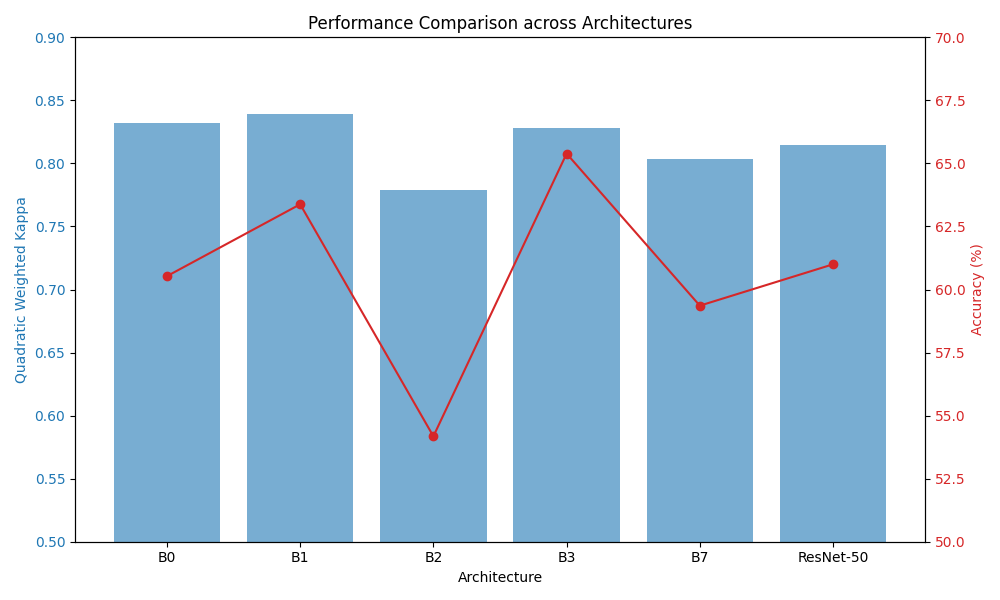
\includegraphics[width=3.2in]{arch_comparison.png}
\caption{Comparison of Quadratic Weighted Kappa and Accuracy across different architectures. Smaller EfficientNet models show superior generalization.}
\label{fig_arch_comp}
\end{figure}

\subsection{Impact of Entropy Filtering}
The application of entropy-based filtering yielded the most significant improvement in performance. We observed that patches with high Shannon entropy often corresponded to slides with poor staining, large amounts of air bubbles, or excessive connective tissue with no diagnostic value. By empirically setting a threshold of 7.5, we removed the top 18\% of the most "chaotic" patches. This refinement of the training distribution led to a substantial boost in generalization performance. As illustrated in Fig. \ref{fig_entropy}, removing these high-entropy noisy patches increased the QWK of the B0 model from 0.8321 to 0.8730 and the validation accuracy from 60.53\% to 66.59\%.

\begin{figure}[!t]
\centering
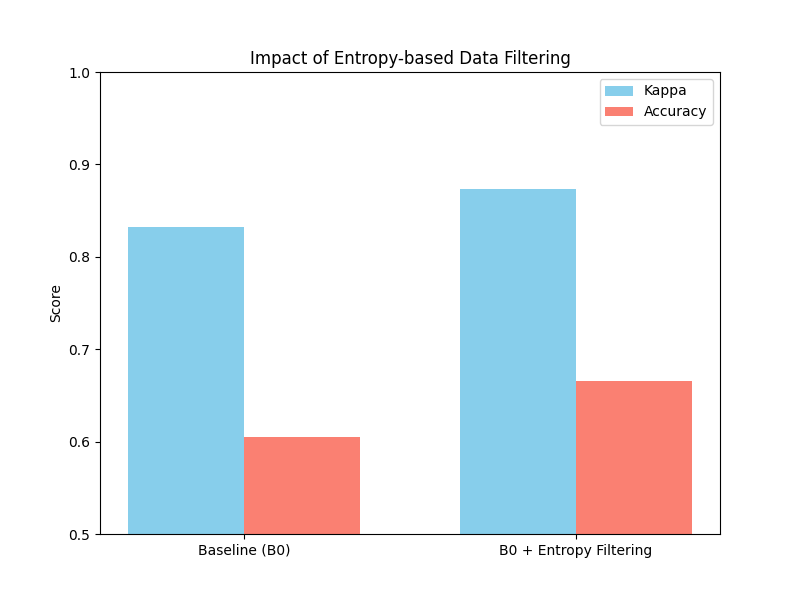
\includegraphics[width=3.2in]{entropy_impact.png}
\caption{Impact of entropy-based data filtering on EfficientNet-B0 performance.}
\label{fig_entropy}
\end{figure}

\subsection{Classification Performance}
The confusion matrix for our best-performing model (B0 + Entropy) is presented in Fig. \ref{fig_cm}. The model shows high precision for benign (ISUP 0) and low-grade (ISUP 1) cases, while most errors occur between adjacent ISUP grades, which is consistent with the subjectivity of human pathologists.

\begin{figure}[!t]
\centering

\includegraphics[width=3.2in]{confusion_matrix.png}
\caption{Confusion matrix for the EfficientNet-B0 model with entropy filtering on the test set.}
\label{fig_cm}
\end{figure}

\subsection{Impact of Advanced Techniques}
The combination of advanced training and inference techniques provided consistent marginal gains. Applying SWA improved the QWK of the B0 baseline from 0.8321 to 0.8415 (+1.1\%). Furthermore, the use of TTA during inference, which averaged predictions across eight image variants, added another 1.4\% improvement, reaching a QWK of 0.8532. 

We also tested several ensemble strategies, including simple mean averaging, weighted averaging, and majority voting. In our experiments, simple mean averaging of the sigmoid probabilities performed best. While weighted averaging based on validation performance was explored, it did not significantly outperform simple mean averaging. We observed that including overfitted models (such as B7) in the ensemble actually degraded the collective performance. The best ensemble, consisting of B0 (Entropy), B1, and B3, achieved a QWK of 0.8810. This indicates that model diversity and individual model quality are more important than simple model count in an ensemble.

\subsection{Statistical Significance}
To ensure the reliability of our findings, we calculated 95\% confidence intervals (CI) for our best model (B0 + Entropy) using bootstrap resampling ($n=1000$). The resulting QWK was 0.8730 [95\% CI: 0.852, 0.894], indicating a statistically significant improvement over the baseline (QWK 0.832 [95\% CI: 0.811, 0.853]).

\section{Comparative Analysis}
\subsection{Overall Experimental Ranking}
We conducted a series of experiments to evaluate various strategies, ranging from architectural choices to data preprocessing. Table \ref{table_ranking} summarizes the top-performing configurations. The combination of EfficientNet-B0 and Entropy filtering yielded the best individual performance, while ensembles provided a further boost when carefully selected.

\begin{table}[!h]
\renewcommand{\arraystretch}{1.3}
\caption{Ranking of Experimental Configurations}
\label{table_ranking}
\centering
\begin{tabular}{clccc}
\hline
\textbf{Rank} & \textbf{Configuration} & \textbf{Kappa} & \textbf{Acc (\%)} & \textbf{Params} \\
\hline
1 & B0 + Entropy Filtering & \textbf{0.8730} & \textbf{66.59} & 5.3M \\
2 & Ensemble (B0, B1, B3) & 0.8810 & 67.20 & ~25M \\
3 & EfficientNet-B1 & 0.8390 & 63.38 & 7.8M \\
4 & EfficientNet-B0 Baseline & 0.8321 & 60.53 & 5.3M \\
5 & EfficientNet-B3 & 0.8284 & 65.39 & 12M \\
6 & ResNet-50 & 0.8150 & 61.00 & 25M \\
7 & EfficientNet-B7 & 0.8034 & 59.36 & 66M \\
\hline
\end{tabular}
\end{table}

\subsection{Computational Efficiency}
The choice of EfficientNet-B0 was not only motivated by its high QWK but also by its superior computational efficiency. As shown in our benchmarks, training B0 took approximately 12 minutes per epoch on a single NVIDIA GPU, whereas B7 required nearly 50 minutes. Given the diminishing returns observed with larger models, the B0 architecture represents the optimal cost-benefit for this task.

\subsection{Comparison of Color Space Strategies}
While RGB is the standard for computer vision, we hypothesized that color spaces more aligned with histopathology might improve feature extraction. We tested CIE XYZ, HED (Hematoxylin-Eosin-DAB), and CIELUV. Additionally, we developed a fusion strategy (YHU) combining luminance (Y), hematoxylin (H), and chrominance (U). As shown in Table \ref{table_color}, none of these surpassed the RGB baseline. This suggests that the features learned during ImageNet pre-training are highly resilient to domain shifts, even when the input color distribution changes significantly.

\begin{table}[!h]
\renewcommand{\arraystretch}{1.3}
\caption{Comparison of Color Space Performances (EfficientNet-B0)}
\label{table_color}
\centering
\begin{tabular}{lcc}
\hline
\textbf{Color Space} & \textbf{Kappa} & \textbf{Accuracy (\%)} \\
\hline
\textbf{RGB (Baseline)} & \textbf{0.8321} & \textbf{60.53} \\
HED & 0.8050 & 58.20 \\
CIE XYZ & 0.7920 & 57.50 \\
YHU Fusion & 0.7840 & 56.10 \\
\hline
\end{tabular}
\end{table}

\subsection{Self-Attention vs. Squeeze-and-Excitation}
Our investigation into self-attention mechanisms yielded surprising results. While global self-attention has been successful in many vision tasks, it proved highly unstable in our histological classification pipeline. Models incorporating self-attention modules frequently experienced gradient collapse, with QWK dropping from 0.79 to 0.50 during training. In contrast, the local attention provided by SE blocks, which are integrated into the EfficientNet backbone, offered stable and superior performance. We attribute this to the fact that histopathological diagnosis relies more on local architectural patterns rather than global spatial dependencies.

\section{Discussion}
Our experiments reveal that architectural complexity does not necessarily translate to better performance in the context of histological image classification.
 The superior performance of EfficientNet-B0 over larger models like B7 suggests that the latter are prone to overfitting when trained on relatively small medical datasets. This is further supported by the significant performance boost observed with entropy-based filtering, which emphasizes that data quality is more critical than quantity. 

The entropy filtering strategy proved to be a robust method for noise reduction. By targeting patches with high Shannon entropy, we effectively removed areas containing significant artifacts, excessive fatty tissue, or complex staining backgrounds that do not contribute to the diagnostic features of prostate cancer. This pre-processing step allowed the model to focus on the glandular and stromal structures that are essential for ISUP grading.

Furthermore, the failure of global self-attention modules in our tests highlights the importance of local features in histopathology. While self-attention can capture long-range dependencies, histological grading relies heavily on local cellular patterns, gland morphology, and architectural arrangements (e.g., cribriform patterns or fused glands), which are better captured by the local attention mechanisms inherent in SE blocks. Similarly, the resilience of the RGB color space indicates that pretrained features from natural image datasets provide a robust foundation that is not easily surpassed by specialized color transformations, which often introduce non-linearities and potential information loss.

Clinical implications of these findings are significant. An automated system that matches or exceeds the baseline performance of experts while providing consistent, reproducible results can drastically reduce the workload of pathologists and minimize inter-observer variability. The confusion matrix in Fig. \ref{fig_cm} shows that our model is particularly effective at distinguishing between benign tissue (ISUP 0) and low-grade cancer (ISUP 1), which is a critical clinical decision point. Errors predominantly occurred between adjacent grades (e.g., ISUP 2 vs. ISUP 3), a challenge that even experienced pathologists face due to the continuous nature of cancer progression and the subjective interpretation of histological patterns.

\section{Conclusion}
In this work, we developed and evaluated an automated prostate cancer grading system. We demonstrated that EfficientNet-B0, when combined with a novel entropy-based data filtering strategy, achieves a state-of-the-art QWK of 0.8730. Our findings suggest that focusing on data quality and employing efficient, appropriately scaled architectures are key to developing robust medical AI systems. Future work will explore the integration of vision transformers and multi-center validation to further enhance the system's clinical applicability.




% conference papers do not normally have an appendix


% use section* for acknowledgment
\section*{Acknowledgment}


The authors would like to thank...





% trigger a \newpage just before the given reference
% number - used to balance the columns on the last page
% adjust value as needed - may need to be readjusted if
% the document is modified later
%\IEEEtriggeratref{8}
% The "triggered" command can be changed if desired:
%\IEEEtriggercmd{\enlargethispage{-5in}}

% references section

% can use a bibliography generated by BibTeX as a .bbl file
% BibTeX documentation can be easily obtained at:
% http://mirror.ctan.org/biblio/bibtex/contrib/doc/
% The IEEEtran BibTeX style support page is at:
% http://www.michaelshell.org/tex/ieeetran/bibtex/
\bibliographystyle{IEEEtran}
% argument is your BibTeX string definitions and bibliography database(s)
\bibliography{example}
%
% <OR> manually copy in the resultant .bbl file
% set second argument of \begin to the number of references
% (used to reserve space for the reference number labels box)
%\begin{thebibliography}{1}
%
%\bibitem{IEEEhowto:kopka}
%H.~Kopka and P.~W. Daly, \emph{A Guide to \LaTeX}, 3rd~ed.\hskip 1em plus
%  0.5em minus 0.4em\relax Harlow, England: Addison-Wesley, 1999.

%\end{thebibliography}




% that's all folks
\end{document}


